% !TeX encoding = UTF-8
% !TeX spellcheck = en_GB
% !TeX root = ../thesis.tex

\chapter{Evaluation and Discussion}
\label{chapter:evaluation}
This chapter evaluates the REPUSH protocol and its proof-of-concept implementation. In doing so, it addresses research question 3 by evaluating the security of the protocol and comparing it to the original PUSH protocol, and it covers research question 4 by measuring the performance of the implementation. 

\section{Security Evaluation}
\subsection{Adversary Model}
The security evaluation follows the threat model outlined in chapter \ref{chapter:design}. The adversary $\Adv$ is assumed to have arbitrary code execution on the host machine. $\Adv$ can read from and write to any memory accessible to the browser and DOMAN, intercept and tamper with inter-process communication, make requests on behalf of the user, and steal session cookies. The communication channel between the browser and the server is also treated as under $\Adv$'s control. However, $\Adv$ is assumed to be incapable of physically interacting with the dongle device and is assumed to computationally be bounded, i.e. unable to break the cryptographic operation within a reasonable time frame.   

This adversary model is stronger than the one considered by the original PUSH protocol \cite{10.1007/978-3-032-07894-0_7}, which only considered browser compromise. REPUSH assumes the entire host is compromised, with the exception of the dongle and server, which are considered as trusted and safe.

\subsection{Resistance to Common Attacks}

\paragraph{Sniffing Attack:}
By monitoring all traffic between protocol parties, $\Adv$ may observe public data such as the challenge issued by the server $C^i_\text{Session}$, $PK_\text{Server}$, cookies, nonces and signed payloads. Notably, the dongle-generated public keys $PK_i$ are never transmitted in plain-text. They are always encrypted so that only the server can decrypt them. None of this data enables $\Adv$ to maintain a session independently of the dongle. Continuing a session requires a periodic validation with a fresh dongle signature, which in turn requires knowledge of $SK_i$, which is never exposed to the host. Moreover, each signature request includes a fresh server-generated nonce that prevents replay attacks.

\paragraph{Cookies Theft and XSS Attacks:} The primary attack against session security is cookie theft, which is carried out by malware (Infostealers). Although XSS was historically a common method for stealing cookies, modern browsers mitigate this through the \verb|HttpOnly| flag, which prevents JavaScript from accessing cookie values directly. The dominant way of stealing cookies is therefore malware which has code execution on the host. In REPUSH, stolen cookies alone are insufficient to hijack a session. Since every time $T_\text{Validity}$ is elapsed, the server requests a fresh signature to verify ownership of the dongle. Without the dongle, $\Adv$ cannot produce the necessary signed payload. The attacker can therefore only use cookies within the $T_\text{Validity}$, and the usage is limited to non-sensitive requests. Real attackers are more interested in using the cookies for sensitive requests like changing passwords and emails, such a sensitive request requires a user-approved dongle signature independent of $T_\text{Validity}$, which makes them inaccessible to $\Adv$.

\paragraph{Replay Attack:}
Each $SignaturePayload$ and $SensitivePayload$ includes a fresh nonce $N$ generated by the server at the time of the request. Even if $\Adv$ records a previously signed payload, replaying it would fail as the server would reject the consumed nonce. Furthermore, the $T_\text{Timeout}$ deadline further restricts the window within which the valid signed payload must arrive at the server.

\paragraph{Man-in-the-Middle (MitM) Attack:}
During phase 1, the dongle verifies the server's certificate using the CA's public key. The verified domain is then displayed on the dongle's screen, where the user must read it and explicitly approve it. A MitM adversary who would use their own certificate must forge the CA's signature, which is infeasible under the assumed adversary model. In subsequent phases, the server signs every payload with $SK_\text{Server}$, so the dongle would only sign payloads coming from the server.

\paragraph{Silent Signing Attack:} The main attack motivating the design of REPUSH is the silent signing attack. In PUSH, $\Adv$ with code execution on the host could silently intercept server-generated payloads and relay them to the dongle via PUFMAN to obtain valid signatures without any user awareness. REPUSH explicitly considers DOMAN as untrusted and addresses this in two ways depending on the type of request. For non-sensitive requests, the dongle verifies the server's signature on $SignaturePayload$ before signing it. $\Adv$ therefore cannot craft an arbitrary payload for the dongle to sign. However $\Adv$ may still intercept the server-generated payload and forward it to the dongle to obtain a signature that it can forward to persist the stolen session. This attack is possible, but only for non-sensitive requests. For sensitive requests, the dongle requires explicit user approval on the dongle display before signing $SensitivePayload$, $\Adv$ can therefore not trigger a silent signature since any attempt to do so would immediately make the user reject it since it would be unsolicited.

\paragraph{Passive Compromise Detection:} A direct consequence of the trusted display requirement for sensitive requests is that REPUSH provides a passive out-of-band indicator of compromise. If any malware attempts to use the dongle to sign a sensitive request that the user did not initiate, an unexpected prompt appears on the dongle's screen, which would immediately alert the user. Because the dongle is isolated from the host and only exposes a limited interface of commands, even the most privileged malware cannot bypass the user-approval on the dongle's screen. This gives the user a reliable way of detecting intrusion independently of any host-based security solution.

\paragraph{Enrollment Hijacking Attack:} In PUSH, if the browser is compromised before enrollment, $\Adv$ could redirect the enrollment to bind the session to their own dongle. REPUSH eliminates this attack by having the dongle independently verify the server certificate and display the domain on the screen for the user to verify it. Furthermore, the credentials are entered on the dongle and not on the browser and are encrypted in transit. A compromised browser can therefore neither alter the domain nor intercept the credentials.

\paragraph{Impersonation Attack:} To impersonate the dongle, $\Adv$ must produce valid signatures to the provided payload using the private key $SK_i$ associated with the currently enrolled public key $PK_i$. This requires knowledge of $SK_i$ which is derived inside the dongle and is never stored on or exposed to the host. Physical access to the dongle could allow the attacker to get $SK_i$, but as mentioned earlier, it is not considered in the attacker model. This limitation will be discussed later in the limitations section. 

\paragraph{Device Capturing and Cloning:}
Although physical attacks are outside our scope, REPUSH's use of an LR-PUF offers many advantages in the case of dongle cloning. Even if the attacker were to steal the dongle and enumerate all the CRPs of the CHOICE-PUF, the attacker would still not be able to predict future keys because the seeds depend on the states as well as the CHOICE-PUF responses, and the states have a TRNG element and time-stamp that determine them. Therefore the attacker would not be able to predict future ($SK_i$,$PK_i$) pairs that the dongle could generate.

\paragraph{Denial-of-Service (DoS) Attack:}
Any party in the REPUSH protocol can be the target of a DoS attack, but the impact is limited to compromising accessibility and no more than that. DoS attacks are less of an issue when it comes to hardware dongles compared to servers, since if that were to occur then that means there is malware on the host. An attacker would have no incentive to just deny service to the dongle since that immediately tells the user that the host is infected.

\section{CHOICE-PUF Evaluation}

In this section, we evaluate the statistical properties of the CHOICE PUF implementation. All measurements were collected via the default serial interface of the FPGA over USB-C at 115200 baud rate. Two datasets were collected. The first dataset is used for uniformity and bit independence evaluation. It consists of one 64-bit response per valid challenge, which gives 184 responses containing a total of $184\times64=11776$ measured bits. The second dataset is used for reliability and error-correction evaluation. It consists of 1000 responses per valid challenge, which gives a total of 184000 measurements. All responses are raw outputs of the PUF before any error correction or majority voting is applied.

\subsection{Uniformity}
A PUF with ideal uniformity produces responses in which each bit is equally likely to be a 0 or a 1. When this property holds, the responses are deemed unpredictable. The ideal uniformity is 50\%, i.e. half of the bits are 0 and the other half are 1. Significant deviations from this ideal indicate a bias on the PUF which could simplify attacks.

\subsubsection{Per-bit Uniformity}
Per-bit uniformity measures the uniformity of each individual bit position across the set of all valid challenges.  For each bit position $b \in \{0, \ldots, 63\}$, the fraction of challenges in which that bit is equal to 1 is computed as:
$$
U_b = \frac{1}{n} \sum_{i=1}^{n} r_i[b]
$$
where $n=184$ is the number of valid challenges and $r_i[b] \in \{0,1\}$ is the $b$-th bit of the $i$-th response. The ideal value is $U_b=0.5$.

The mean per-bit uniformity $\bar{U}_\text{per-bit}$ is the mean of $U_b$ over all bits, which is computed as:
$$
    \bar{U}_\text{per-bit} = \frac{1}{64} \sum_{b=0}^{63} U_b
$$

The measured mean per-bit uniformity is $\bar{U}_\text{per-bit}=51.04\%$, which is very close to the ideal $50\%$.

The mean absolute deviation (MAD) measures on average how far each bit position deviates from the ideal uniformity:
$$
MAD = \frac{1}{64}\sum_{b=0}^{63}|U_b - 0.5|
$$

The measured MAD is $MAD=6.33\%$.

Figure \ref{fig:per-bit-uniformity} shows the per-bit uniformity for all 64 bit positions. The bars in red deviate by 10 percentage points or more from the ideal 50\% uniformity.

\begin{figure}
    \centering
    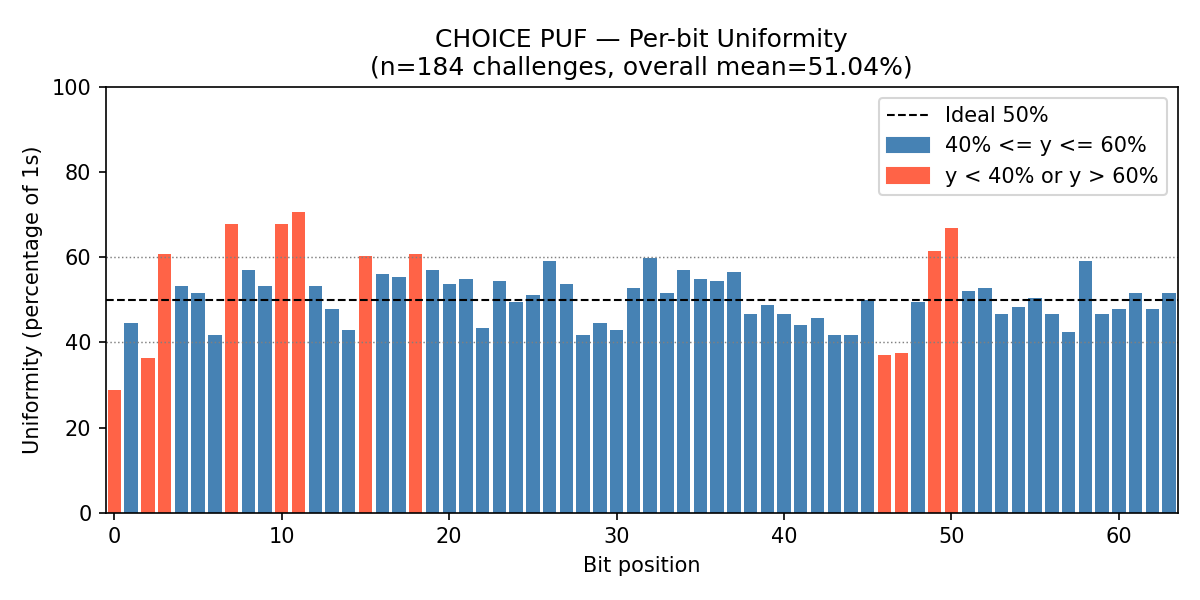
\includegraphics[width=1\linewidth]{img/plot_uniformity_bits.png}
    \caption{CHOICE-PUF: Per-bit Uniformity.}
    \label{fig:per-bit-uniformity}
\end{figure}

The most biased bit is bit position 0, which equals 1 in only 28.8\% of responses. But overall, the other bits are well balanced. Per-bit uniformity captures whether bit positions are uniform across all challenges, but it does not reveal whether individual responses are uniform. The next section addresses this. 

\subsubsection{Per-challenge Uniformity}
Per-challenge uniformity measures the Hamming weight of each 64-bit response as:
$$
U_i = \frac{1}{64}\sum_{b=0}^{63} r_i[b]
$$
where $r_i[b] \in \{0,1\}$ is the $b$-th bit of response $r_i$. The ideal value is $U_i=0.5$ for every challenge. 

The mean per-challenge uniformity $\bar{U}$ is the mean of $U_i$ over all responses, which is computed as:
$$
\bar{U} = \frac{1}{n}\sum_{i=1}^{n} U_i
$$
where $n = 184$ is the number of valid challenges. It was measured as $\bar{U}=51.04\%$.

The per-challenge MAD measures on average how far each individual response deviates from the ideal uniformity:
$$
MAD_\text{per-challenge} = \frac{1}{n}\sum_{i=1}^{n}|U_i - 0.5|
$$

The measured value is $MAD_\text{per-challenge} = 27.86\%$

Figure \ref{fig:per-challenge-uniformity}  shows the per-challenge uniformity sorted in ascending order. Only 22 out of the 184 challenges (12\%) fall near the ideal 50\% uniformity; those are highlighted in blue on the figure. Despite the ideal-looking mean uniformity, the responses are in majority quite far from the mean as can be seen with the red bars. This shows that the CHOICE PUF alone is not a reliable source of uniform responses, with 88\% of challenges producing outputs far from the ideal. Naively selecting a challenge at random would most likely yield a biased response. This reinforces the need for the LR-PUF construction to augment the CHOICE-PUF's responses using hashing with random states.

\begin{figure}
    \centering
    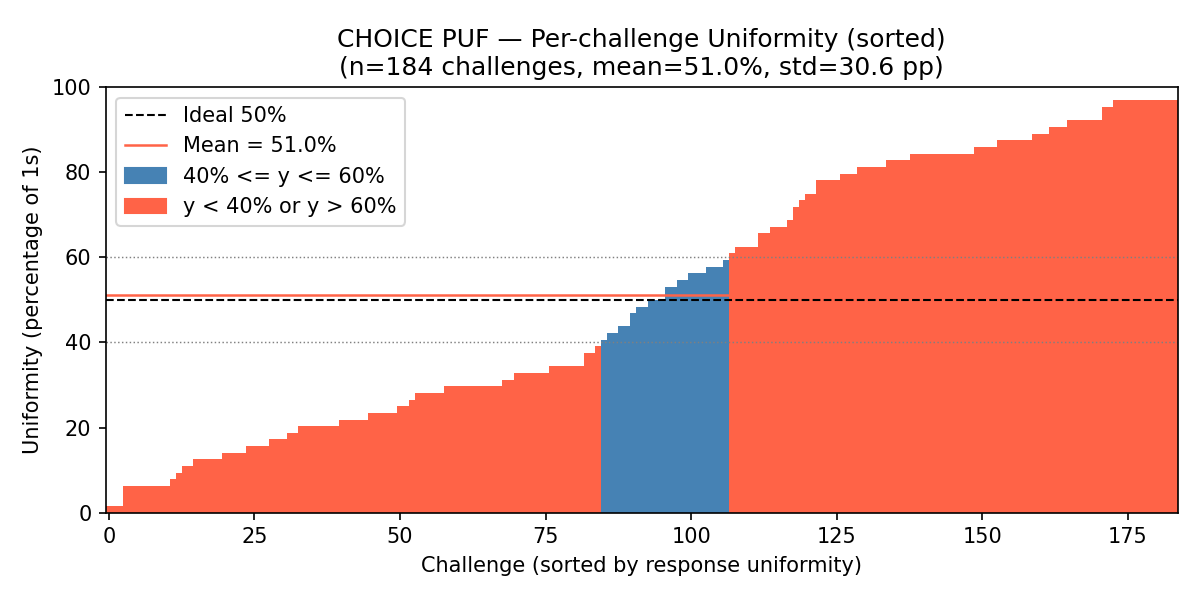
\includegraphics[width=1\linewidth]{img/plot_uniformity_per_challenge.png}
    \caption{CHOICE-PUF: Per-challenge Uniformity}
    \label{fig:per-challenge-uniformity}
\end{figure}

Table \ref{tab:uniformity-results} summarizes the uniformity results. $\bar{U}$ and $\bar{U}_\text{per-bit}$ are identical by definition. The mean absolute values however differ. $MAD_\text{per-challenge} = 27.86\%$ is much bigger than $MAD_\text{per-bit}=6.33\%$. This shows that individual bit positions are moderately balanced whilst individual bit sequences are heavily skewed. 

\begin{table}[ht!]
\centering
\caption{CHOICE PUF uniformity results summary.}
\begin{tabular}{llll}
\hline
\textbf{Metric} & \textbf{Symbol} & \textbf{Measured} & \textbf{Ideal} \\
\hline
Mean per-bit uniformity            & $\bar{U}_\text{per-bit}$      & 51.04\%          & 50\%  \\
MAD per-bit                               & $MAD_\text{per-bit}$   & 6.33\%         & 0\% \\
Bit positions within $\pm10\%$\   & —                             & 52 / 64 (81\%)   & 100\% \\
Bit positions outside $\pm10\%$  & —                             & 12 / 64 (19\%)   & 0\%   \\
\hline
Mean per-challenge uniformity      & $\bar{U}$                           & 51.04\%          & 50\%  \\
MAD per-challenge                              & $MAD_\text{per-challenge}$   & 27.86\%        & 0\% \\
Challenges within $\pm10\%$      & —                                   & 22 / 184 (12\%)  & 100\% \\
Challenges outside $\pm10\%$     & —                                   & 162 / 184 (88\%) & 0\%   \\
\hline
\end{tabular}
\label{tab:uniformity-results}
\end{table}

\subsection{Uniqueness}

Uniqueness measures how distinct the responses of two or more different PUF instances are when presented with the same challenge. The standard metric for measuring uniqueness is the inter-device Hamming distance, which has an ideal value of 50\%, meaning that two independent devices agree on exactly half of the bits by randomness. A score significantly below 50\% indicates that responses are too similar across devices, which would allow one device to impersonate another.

Measuring inter-device uniqueness requires multiple FPGA chips flashed with the PUF design, which is impractical for this thesis. To circumvent this limitation, the 64-bit response is split into two 32-bit responses $r^{lo}$ and $r^{hi}$, and the two responses are treated as coming from two different devices. For each challenge $i$, the inter-device Hamming distance is computed as:
$$
D_i = \frac{1}{32}\sum_{b=0}^{31} \left| r_i^\text{hi}[b] - r_i^\text{lo}[b] \right|
$$
where $r_i^\text{hi}[b]$ and $r_i^\text{lo}[b]$ are the $b$-th bit of each half.

The mean uniqueness score $\bar{D}$ is averaged across all $n = 184$ challenges:
$$
\bar{D} = \frac{1}{n} \sum_{i=1}^{n} D_i
$$

The measured mean uniqueness is $\bar{D} = 29.50\%$.

The mean absolute deviation of the uniqueness from the ideal is:
$$
MAD_\text{uniqueness} = \frac{1}{n} \sum_{i=1}^{n} |D_i - 0.5|
$$

The measured value is $MAD_\text{uniqueness} = 21.28\%$

Figure \ref{fig:uniqueness} shows the inter-device Hamming distance for each challenge sorted in ascending order. Only 53 out of the 184 valid challenges (28.8\%) fall near the ideal 50\% uniqueness, which tells us that the two halves do not fully behave as two different devices.

\begin{figure}
    \centering
    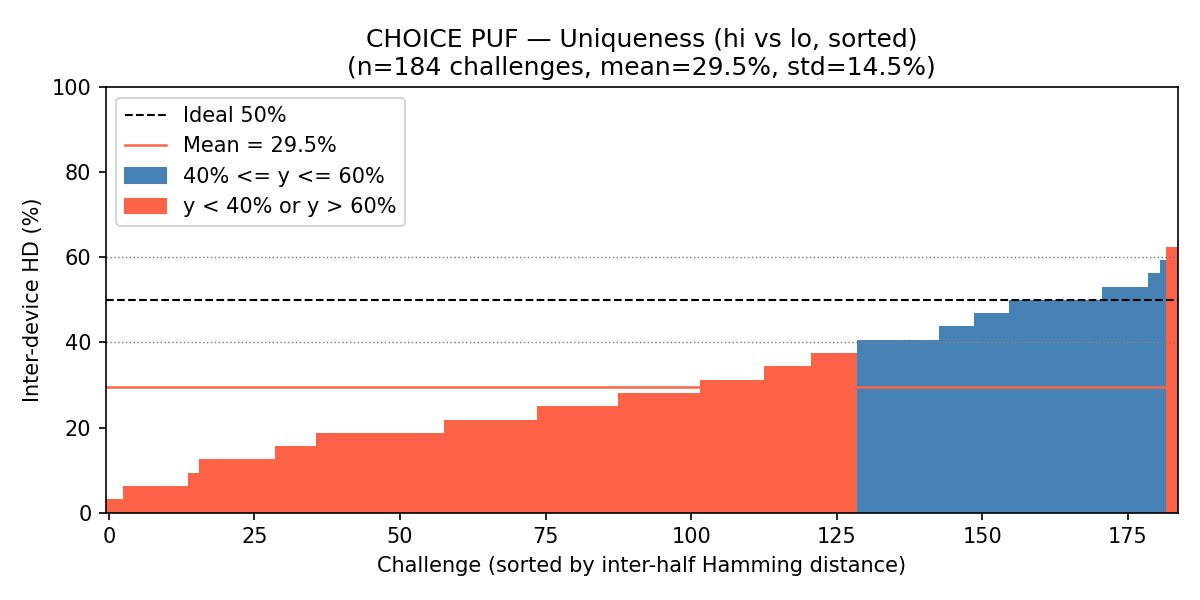
\includegraphics[width=1\linewidth]{img/plot_uniqueness.png}
    \caption{CHOICE-PUF: Uniqueness}
    \label{fig:uniqueness}
\end{figure}

Table \ref{tab:uniqueness-results} summarizes the uniqueness results. The mean uniqueness of $\bar{D} = 29.50\%$ is well below the ideal of 50\%, and the large $MAD_\text{uniqueness} = 21.28\%$ confirms that individual challenges deviate substantially from the ideal. This is explained by the structural proximity of the two halves on the FPGA. This measurement can therefore only be considered as a lower bound rather than a true inter-device uniqueness score. A rigorous evaluation would require measuring uniqueness over many boards.


\begin{table}[ht!]
\centering
\caption{CHOICE PUF uniqueness results summary.}
\begin{tabular}{llll}
\hline
\textbf{Metric} & \textbf{Symbol} & \textbf{Measured} & \textbf{Ideal} \\
\hline
Mean inter-half distance           & $\bar{D}$                         & 29.50\%          & 50\%  \\
MAD                                & $MAD_\text{uniqueness}$           & 21.28\%          & 0\%   \\
Challenges within $\pm10\%$        & —                                 & 53 / 184 (29\%)  & 100\% \\
Challenges outside $\pm10\%$       & —                                 & 131 / 184 (71\%) & 0\%   \\
\hline
\end{tabular}
\label{tab:uniqueness-results}
\end{table}




\subsection{Reliability}
Reliability measures how consistently a PUF produces the same response when queried with the same challenge under the same conditions. A PUF usually produces slightly different responses on each query due to changing conditions. For the REPUSH protocol, reliability is important since the BCH fuzzy commitment scheme can only tolerate up to $T=4$ bit flips between the enrollment response and the query response. If the PUF produces more than 4 flipped bits, BCH decoding will fail, and the key cannot be reconstructed.

The reliability metric used is the one from the pypuf python library \cite{nils_wisiol_2021_5222515}. Each challenge is queried $r$ times, producing $r$ 64-bit responses. Let $\hat{p}_b$ be the fraction of $r$ responses in which bit position $b$ equals 1. The reliability of bit $b$ under some challenge is:
$$
\rho_b = \hat{p}_b^2 + (1-\hat{p}_b)^2 = 1 - 2\hat{p}_b(1-\hat{p}_b) = 1 - 2\,\mathrm{Var}(\hat{p}_b)
$$

$\rho_b$ is the probability that two independent queries of the same challenge agree on bit $b$. Both queries return 1 with probability $\hat{p}_b^2$ and both return 0 with probability $(1-\hat{p}_b)^2$. After expanding this expression we get $\rho_b = 1 - 2\hat{p}_b(1-\hat{p}_b)$ where $\hat{p}_b(1-\hat{p}_b)$ is the variance of a binary random variable. Reliability is simply 1 minus twice the observed variance of the bit. A perfectly stable bit ($\hat{p}_b \in \{0,1\}$) gives $\rho_b = 1$ and a maximally noisy bit ($\hat{p}_b = 0.5$) gives $\rho_b = 0.5$.

The dataset has $r=1000$ samples per challenge across all $n=184$ valid challenges. The responses are arranged into an $(n \times 64 \times r)$ array. For each of the challenge-bit pairs, $\hat{p}_b$ is computed as the fraction of 1s across the $r=1000$ queries. Then $\rho_b$ is computed using the formula above. The result is an $(n \times 64)$ reliability matrix which gives the reliability of each bit given a challenge.

From the reliability matrix, we compute the per-bit reliability by averaging the reliability for each bit $b$ over all $n$ challenges:

$$
\bar{\rho}_b = \frac{1}{n} \sum_{i=1}^{n} \rho_{i,b}
$$

As seen in figure \ref{fig:reliability-per-bit}, the least reliable bit is bit position 1 with a reliability of 98.39\%. The majority of bit positions have above 99\% reliability which indicates that the CHOICE-PUF is very reliable.

\begin{figure}
    \centering
    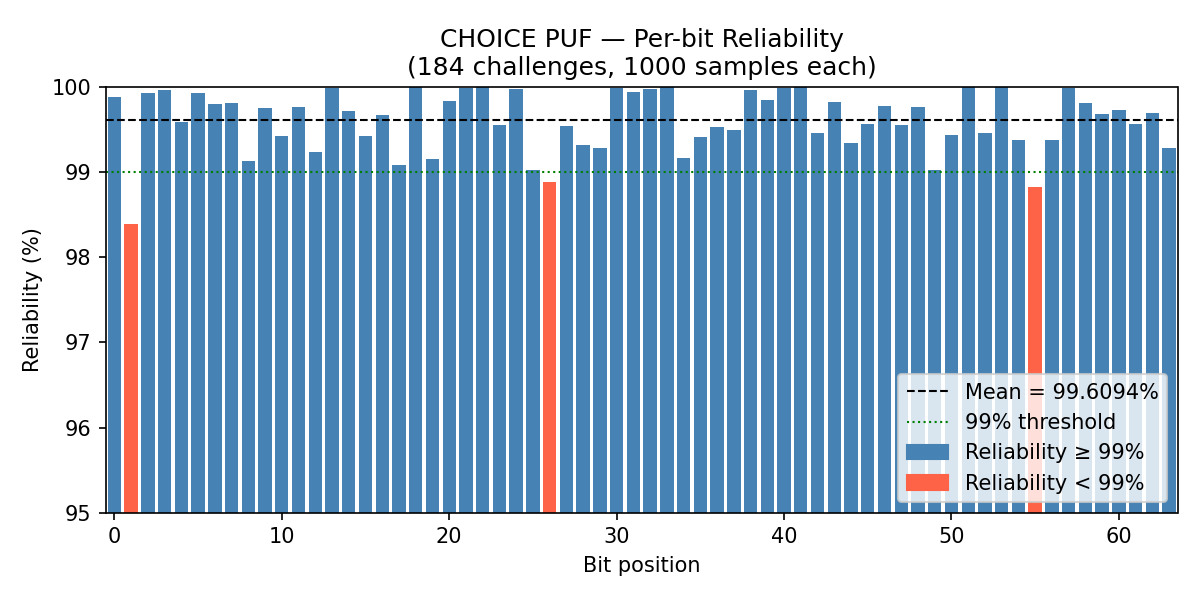
\includegraphics[width=1\linewidth]{img/plot_reliability_per_bit.png}
    \caption{CHOICE-PUF: Per-bit Reliability}
    \label{fig:reliability-per-bit}
\end{figure}

Alternatively, the per-challenge reliability can be computed by averaging over all 64 bits for each challenge to give one reliability value per challenge $i$:

$$
\bar{\rho}_i = \frac{1}{64} \sum_{b=0}^{63} \rho_{i,b}
$$

As seen in figure \ref{fig:reliability-per-challenge}, the least reliable challenge has a reliability of 97.41\%, whilst most challenges are well above 99\%. 

\begin{figure}
    \centering
    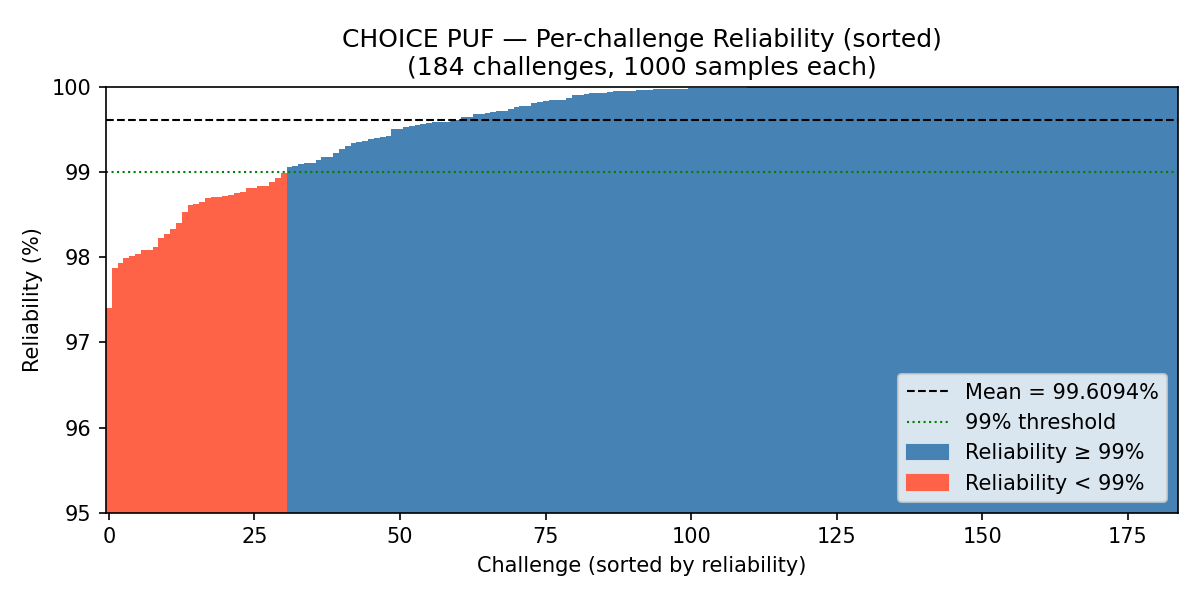
\includegraphics[width=1\linewidth]{img/plot_reliability_per_challenge.png}
    \caption{CHOICE-PUF: Per-challenge Reliability}
    \label{fig:reliability-per-challenge}
\end{figure}

The overall reliability $\bar{\rho}$ is the average of all values within the reliability matrix: 
$$
\bar{\rho} = \frac{1}{64n} \sum_{i=1}^{n} \sum_{b=0}^{63} \rho_{i,b}
$$
The measured value for the overall reliability is $\bar{\rho}=99.61\%$

Table \ref{tab:reliability-results} summarizes the reliability results.

\begin{table}[ht!]
\centering
\caption{CHOICE PUF reliability results summary.}
\begin{tabular}{llll}
\hline
\textbf{Metric} & \textbf{Symbol} & \textbf{Measured} & \textbf{Ideal} \\
\hline
Overall reliability              & $\bar{\rho}$          & 99.61\%   & 100\% \\
Least reliable bit (bit 1)       & $\min_b \bar{\rho}_b$ & 98.39\%   & 100\% \\
Least reliable challenge (idx 99)& $\min_i \bar{\rho}_i$ & 97.41\%   & 100\% \\
\hline
\end{tabular}
\label{tab:reliability-results}
\end{table}

\section{LR-PUF Evaluation}

The statistical properties of the CHOICE-PUF evaluated in the previous section carry directly over to the LR-PUF. The high $99.61\%$ reliability of the CHOICE-PUF ensures that the BCH fuzzy commitment can consistently reconstruct the same seed across repeated queries since the expected number of bit flips per query is within the $T=4$ correction capacity. The poor per-challenge uniformity of the CHOICE-PUF responses, where 88\% of the challenges are 10\% far from the ideal 50\% uniformity, is fixed by the BLAKE2b hash that is applied on the CHOICE-PUF responses since by definition a cryptographic hash function produces uniform outputs regardless of the bias in its inputs. Therefore, the 32-byte seed derived from the LR-PUF is uniformly distributed. The LR-PUF inherits the reliability of the CHOICE-PUF while eliminating its uniformity limitations through hashing. Inter-state uniqueness within one device is guaranteed by the random seed that is used to generate each state. But inter-device uniqueness remains dependent on the CHOICE-PUF producing distinct responses on different FPGA chips, which we could not fully verify.

\subsection{TRNG Evaluation}
A critical piece to the LR-PUF is the TRNG used for generating the initial state. In the implementation, a seed is generated from an unconnected pin on the Arduino. It is therefore essential to evaluate the randomness of the outputs generated by this method. To assess the quality of this source, 125\,000 bytes (1\,000\,000 bits) were collected and evaluated using the NIST SP800-90B non-IID entropy assessment tool (\cite{nist_sp800_90b} and \cite{sp800_90b_entropy_assessment}).

Min-entropy $H$ represents the worst-case unpredictability of a random source. It describes the unpredictability of an outcome determined solely by the probability of the most likely result \cite{crypto_se_63797}. It is defined as:
$$
H = -\log_2(p_{\max})
$$

where $p_{\max}$ is the probability of the most likely output value.

For example, if we have an algorithm that produces 8-digit passwords, if the number \verb|00000000| occurs 50\% of the time, and the remaining $10^8-1$ passwords occur with equal probability, then the min-entropy is $H=-\log_2(P(X=\texttt{00000000}))=-\log_2(0.5)=1$.
Equivalently, $p_{\max} = 2^{-H}$. Therefore a min-entropy of 1 means that there is a 50\% chance that a single guess gets the right password. Whilst a min-entropy of 8 means only 1 in 256 guesses would get it right ($H = -\log_2\left(\tfrac{1}{256}\right) = -\log_2(2^{-8}) = 8$). This assumes the attacker knows the distribution and exploits it. Rather than enumerating passwords at random, the attacker always guesses \texttt{00000000} first and succeeds 50\% of the time in a single try. If the distribution were perfectly uniform, no single guess would be better than any other and the min-entropy would be $-\log_2(1/10^8) \approx 26.6$ bits, which means that even an optimal attacker only has a 1-in-100-million chance on the first guess.

The NIST SP800-90B non-IID entropy assessment tool assesses this entropy. It does so under the non-IID assumption. IID stands for independent and identically distributed. A source is IID if every sample is drawn independently from the same fixed distribution. For example, throwing a coin is an IID source since one coin toss does not influence the next in any way. But the successive readings of a floating Arduino pin are non-IID since every reading is somewhat influenced by the previous one. The assessment tool therefore does not assume that the entropy source is IID and applies many tests to estimate the min-entropy.

The tool produced the following estimates:
\begin{itemize}
    \item $H_\text{original}=7.571$ bits per byte. The tool was told that each sample is 8 bits long, so it treats each byte as a single symbol and estimates its min-entropy. A perfectly random byte would have $H_\text{original}=8$ bits, i.e. each of the 256 values is equally likely. The measured value of 7.571 means that the source provides   $\frac{7.571}{8}\cdot100\%=94.6\%$ of that 8-bit maximum.
    \item $H_\text{bitstring}=0.825$ bits per bit. Here, each bit is considered as a symbol rather than the entire byte. A perfectly random bit would have $H_\text{bitstring}=1$ bit, i.e. an equal probability of 1 and 0 ($p_{\max}=0.5$). The measured value of 0.825 means $p_{\max} = 2^{-0.825} \approx 0.567$, so the tool can predict the next bit correctly $56.7\%$ of the time using its predictors. This is only possible if the predictors find some sort of pattern in the previous bits, which means that consecutive bits are not fully independent from each other.    
\end{itemize}

To compare these two estimates and get a more conservative minimum entropy, $H_\text{bitstring}$ is multiplied by 8 to convert it to "bits per byte" $8\cdot H_\text{bitstring}=6.603$ and the minimum of the two measured values is taken as the actual min-entropy:
$$
H=  \min\!\left(H_\text{original},\ 8 \times H_\text{bitstring}\right) = \min(7.571,\ 6.603) = 6.603 \text{ bits/byte.}
$$


The 32-byte seed generated by the TRNG for initializing the LR-PUF state therefore carries around $32 \cdot 6.603 \approx 211$ bits of min-entropy. The theoretical maximum would be 256 bits of min-entropy. Despite falling short of full entropy, the 211 bits of min-entropy are usable for cryptographic purposes, since an optimal adversary who exploits the full distribution of the source succeeds with probability of at most $2^{-211}=3.04\times10^{-64}$.

Table \ref{tab:trng-results} summarizes the findings.

It should be noted that the SP800-90B standard recommends a minimum of 1\,000\,000 bytes of measurements for getting statistically meaningful results, whereas we only collected 125\,000 bytes due to the low throughput of using \texttt{analogRead} for the TRNG ($\approx$15\,bytes per second).

\begin{table}[h]
\centering
\caption{NIST SP\,800-90B entropy assessment results for the Arduino floating-pin TRNG.}
\begin{tabular}{lcc}
\hline
\textbf{Metric} & \textbf{Measured} & \textbf{Ideal} \\
\hline
$H_\text{original}$ (bits/byte) & 7.571 & 8 \\
$H_\text{bitstring}$ (bits/bit) & 0.825 & 1 \\
$8 \times H_\text{bitstring}$ (bits/byte) & 6.603 & 8 \\
$H = \min(H_\text{original},\ 8 \times H_\text{bitstring})$ (bits/byte) & \textbf{6.603} & 8 \\
Total min-entropy for 32-byte seed (bits) & $\approx 211$ & 256 \\
\hline
\end{tabular}
\label{tab:trng-results}
\end{table}

\section{Performance Evaluation}
\subsection{LR-PUF Performance}
To measure the performance of the LR-PUF implementation, latency was measured from the host computer using a Python script that communicates with the FPGA via its default serial interface of USB-C at 115200 baud rate. To record the time taken, the start time is taken from the moment the command was transmitted until the final response line is received. The reported measurements therefore include a small additional delay introduced by the UART communication.

\subsubsection{BCH Enroll}

Each enrollment sample covers the total time for the following major operations:
\begin{itemize}
    \item $1\times$ BLAKE2b hash: for running the $map_{in}$ function.
    \item $10\times$ CHOICE-PUF query: to do majority voting and get a stable CHOICE-PUF response.
    \item $1\times$ BLAKE2b hash: to derive the fuzzy commitment secret $W$.
    \item $1\times$ BCH encode: to compute $ECC$ parity bits for $W$.
    \item $1\times$ SD block write: to persist $ECC$ and helper data.
    \item $1\times$ BLAKE2b hash: to derive the final 32-byte seed.
\end{itemize}

Thirty samples were collected to get the results shown in table \ref{tab:perf-bch-enroll}. 
\begin{table}[ht!]
\centering
\caption{BCH enrollment latency ($n=30$).}
\begin{tabular}{lc}
\hline
\textbf{Metric} & \textbf{Measured} \\
\hline
Minimum      & 48.7 ms \\
Maximum      & 52.4 ms \\
Mean         & 50.5 ms \\
Median       & 50.6 ms \\
Std. dev.  &  0.9 ms \\
\hline
\end{tabular}
\label{tab:perf-bch-enroll}
\end{table}

The median enrollment latency is 50.6 ms. Since this operation is an operation that only happens at login and at session renewal, its latency has no significant impact on the user experience.

\subsubsection{BCH Query}
Each query sample covers the total time for the following major operations:
\begin{itemize}
    \item $1\times$ BLAKE2b hash: for running the $map_{in}$ function.
    \item $1\times$ CHOICE-PUF query.
    \item $1\times$ BCH decode: to correct eventual bits flips to reconstruct $W$.
    \item $1\times$ BLAKE2b hash: to derive the 32-byte seed.
\end{itemize}

Fifty samples were collected to get the results shown in table \ref{tab:perf-bch-query}.

\begin{table}[ht!]
\centering
\caption{BCH query latency ($n=50$).}
\begin{tabular}{lc}
\hline
\textbf{Metric} & \textbf{Value} \\
\hline
Minimum      & 24.2 ms \\
Maximum      & 26.7 ms \\
Mean         & 24.8 ms \\
Median       & 24.7 ms \\
Std dev  &  0.6 ms \\
\hline
\end{tabular}
\label{tab:perf-bch-query}
\end{table}

The median query latency is 24.7 ms. The query operation runs many times throughout the session to generate the seed for the key to sign the incoming payload. This latency would be imperceptible to the user. As will be seen in the next sections, the bulk of the latency is not from the LR-PUF, but rather from the cryptographic operations needed for the protocol.

\subsection{Phase 1 Performance}

The enrollment time contains the dongle's enrollment operation, the server's cryptographic verification and the finally the dongle's acknowledge operation. Since this phase relies on user interaction to accept the login request and enter the username and password, this user interaction time was subtracted from the measurements. Three components of the enrollment flow were timed across ten trials.

The measured dongle enrollment operation contains the following operations, excluding the user interaction:
\begin{itemize}
    \item $2\times$ Ed25519 verification: for verifying the server certificate and the enroll payload signature.
    \item FPGA requests: to find a free state slot, reconfigure it, generate a seed and enroll it using BCH, assign the domain to the selected state and persist the state to the SD card.
    \item $1\times$ Ed25519 key derivation: for deriving the dongle's public key and from the seed.
    \item $1\times$ X25519 key agreement: ephemeral ECDH with the server's public key to get a key for encrypting the username, password and dongle public key.
    \item $1\times$ ChaCha20-Poly1305 encryption: to encrypt the username, password and dongle public key so that only the server can decrypt it.
    \item $1\times$ Ed25519 signature: signing the enroll payload using the dongle's generated private key.
\end{itemize}

The server verification operation occurs after the server receives the login token from the dongle, it contains the following operations:
\begin{itemize}
    \item $1\times$ X25519 key agreement: ECDH with the dongle's ephemeral public key to generate the shared key for decrypting the token.
    \item $1\times$ ChaCha20-Poly1305 decryption: to recover the encrypted user credentials and the dongle's enrolled public key.
    \item $1\times$ Ed25519 verification: to validate the signature on the enroll payload.
    \item $1\times$ Credential hashing: to verify the password.
    \item $1\times$ Ed25519 signature: to produce the acknowledgment token.
\end{itemize}

The dongle acknowledgment operation occurs after the dongle receives the acknowledgment token from the server. It contains the following operations:
\begin{itemize}
    \item $1\times$ FPGA requests: to get the state associated with domain, the stored device public key, challenge, and server public key.
    \item $1\times$ Ed25519 verification: to validate the server's acknowledgment signature.
    \item $1\times$ FPGA request: to mark the state slot as acknowledged.
\end{itemize}

Table \ref{tab:perf-phase1} summarizes the measurements.

\begin{table}[ht!]
\centering
\caption{Phase 1 enrollment latency ($n=10$).}
\begin{tabular}{lrrrrr}
\hline
\textbf{Operation} & \textbf{Min} & \textbf{Max} & \textbf{Mean} & \textbf{Median} & \textbf{Std. dev.} \\
\hline
Dongle enroll (ms)      & 8\,828 & 13\,169 & 9\,928 & 8\,880 & 1\,520 \\
Server verify (ms)      &   282  &    464  &   307  &   291  &    56  \\
Dongle acknowledge (ms) & 1\,832 &  1\,870 & 1\,851 & 1\,852 &    12  \\
\hline
\end{tabular}
\label{tab:perf-phase1}
\end{table}

Overall, the entire phase 1 takes on average 12 seconds. When it comes to user experience, 12 seconds is acceptable for such a one-time operation that only occurs at every login.

\subsection{Phase 2 Performance}

Both sensitive and non-sensitive signing execute the same cryptographic operations on the dongle and the server. The only difference is that the sensitive signing requires user approval. This user interaction time is therefore excluded from the measurements. Ten trials were collected for each variant of phase 2.

To assess the performance of the continuous validation, three components of the signing flow were timed across ten trials.

The measured dongle signing operation contains the following operations:
\begin{itemize}
    \item $1\times$ FPGA requests: to get the state associated with the domain, the stored device public key and the server public key.
    \item $1\times$ Ed25519 verification: to validate the signature payload.
    \item $1\times$ FPGA request: for BCH fuzzy commitment querying to reconstruct the dongle's enrolled private key via the LR-PUF.
    \item $1\times$ Ed25519 signature: to sign the signature payload with the reconstructed private key.
\end{itemize}

The server signature verification operation includes one Ed25519 verification to validate that the received payload from the dongle corresponds to the enrolled public key.

For non-sensitive signing, the round trip is additionally measured on the server-side from the time the signing operation is issued until the signed payload is received and verified by the server. It is what the user would perceive in terms of delay.

Table \ref{tab:perf-phase2} summarizes all measurements.

\begin{table}[ht!]
\centering
\caption{Phase 2 signing latency by component ($n=10$; sensitive dongle sign excludes user interaction).}
\begin{tabular}{llrrrrr}
\hline
\textbf{Variant} & \textbf{Operation} & \textbf{Min} & \textbf{Max} & \textbf{Mean} & \textbf{Median} & \textbf{Std. dev.} \\
\hline
\multirow{3}{*}{Non-sensitive}
  & Dongle sign (ms)   & 2\,778 & 2\,863 & 2\,815 & 2\,814 & 25 \\
  & Server verify (ms) &   0.94 &   2.48 &   1.60 &   1.37 & 0.52 \\
  & Round trip (s)     &  4.331 &  4.428 &  4.372 &  4.364 & 0.031 \\
\hline
\multirow{2}{*}{Sensitive}
  & Dongle sign (ms)   & 2\,764 & 2\,847 & 2\,810 & 2\,804 & 25 \\
  & Server verify (ms) &   0.68 &   2.63 &   1.32 &   1.07 & 0.65 \\
\hline
\end{tabular}
\label{tab:perf-phase2}
\end{table}

The user-perceived delay is around 4.4 seconds for non-sensitive signing. Most of it is dominated by the cryptographic operations carried on the dongle. The signing and verification operations performed by the Arduino are very slow: it takes around 1675 ms for the Ed25519 verification and 1045 ms for the Ed25519 signing. The dongle sign times and server verification times for sensitive and non-sensitive requests are very similar since the same operations occur. 

\subsection{Phase 3 Performance}
Phase 3 is triggered when the session expires to generate new keys. It requires user-approval on the dongle to extend the session. Therefore, the user interaction time is subtracted from the dongle reconfiguration measurement. Ten trials were collected.

The dongle reconfiguration operation contains the following operations:
\begin{itemize}
    \item $1\times$ FPGA requests: to get state associated with the domain, the stored device public key and the server public key.
    \item $1\times$ Ed25519 verification: to validate the server's signature on the reconfiguration payload.
    \item $1\times$ FPGA request: for BCH fuzzy commitment querying to reconstruct the current private key.
    \item $1\times$ FPGA request: to reconfigure the state associated with the domain.
    \item $1\times$ FPGA request: to enroll a new key using BCH fuzzy commitment with the new reconfigured state.
    \item $1\times$ Ed25519 signature: to sign the reconfiguration payload.
    \item $1\times$ X25519 key agreement: ECDH with the server's public key.
    \item $1\times$ ChaCha20-Poly1305 encryption: to encrypt the reconf token so that only the server can decrypt it.
    \item $1\times$ FPGA requests: to persist the new enrollment.
\end{itemize}

The server verification operation includes the following:
\begin{itemize} 
    \item $1\times$ X25519 key agreement: ECDH with the dongle's ephemeral public key.
    \item $1\times$ ChaCha20-Poly1305 decryption: to decrypt the reconf token.
    \item $1\times$ Ed25519 verification: to verify the dongle's signature on the reconfiguration payload.
    \item $1\times$ Ed25519 signature: to produce the reconfiguration acknowledgment. 
\end{itemize}

The dongle acknowledgment operation includes:
\begin{itemize}
    \item $1\times$ FPGA requests: to get the state associated with the domain that contains the newly enrolled public key.
    \item $1\times$ Ed25519 verification: to verify the server's acknowledgment signature.
    \item $1\times$ FPGA request: to mark the state as acknowledged. 
\end{itemize}

Table \ref{tab:perf-phase3} summarizes the results.

\begin{table}[ht!]
\centering
\caption{Phase 3 reconfiguration latency ($n=10$).}
\begin{tabular}{lrrrrr}
\hline
\textbf{Operation} & \textbf{Min} & \textbf{Max} & \textbf{Mean} & \textbf{Median} & \textbf{Std. dev.} \\
\hline
Dongle reconf (ms) & 8\,892 & 8\,920 & 8\,904 & 8\,902 &  9.7 \\
Server verify (ms) &   1.19 &  24.67 &   9.48 &   7.77 &  7.3 \\
Dongle ack (ms)    & 1\,853 & 1\,911 & 1\,887 & 1\,892 & 18.0 \\
\hline
\end{tabular}
\label{tab:perf-phase3}
\end{table}

The reconfiguration phase takes on average 11 seconds, which is very similar to phase 1 since both phases have many operations in common. Since this phase only occurs when the session expires, 11 seconds is acceptable in terms of user experience.


\section{Comparison with the PUSH Protocol}
This sections provides a comparison between PUSH \cite{10.1007/978-3-032-07894-0_7} and REPUSH.

\subsection{Threat Model}
The most fundamental distinction between the two protocols is the threat model. PUSH treats PUFMAN and the dongle as fully trusted, and only considers the browser as a potentially compromised party (e.g. through a malicious browser extension). It also considers that the browser is not compromised prior to the enrollment phase. An attacker who achieves general remote code execution on the host falls outside of the scope of the PUSH threat model.

REPUSH extends the threat model by assuming that the entire host is potentially compromised. Only the dongle and server are treated as trusted parties. This stronger model is motivated by two attacks that are possible when the host is trusted.

\subsubsection{Silent Signing Attack}
The first is the silent signing attack where the attacker could impersonate PUFMAN and act as a proxy to the dongle to get the valid signatures and maintain the stolen session. REPUSH partially addresses this by requiring explicit user approval on the dongle's touch screen for sensitive requests, which makes silent signing of those impossible. However, for non-sensitive requests, a compromised DOMAN can still intercept a server-generated $SignaturePayload$ and relay it to the dongle, which will verify the server's signature and sign it without any user interaction. Silent signing of non-sensitive requests is possible in REPUSH, but the impact is limited compared to PUSH. 

\subsubsection{Enrollment Hijacking}
The second motivation is the enrollment hijacking attack. In PUSH, the user manually provides a manufacturer-issued dongle public key to the browser during enrollment. The browser uses this key during enrollment to verify if some signatures coming from the dongle are legitimate before forwarding them to the server. If the attacker has access to the browser during or before enrollment, then this mechanism is under their control, as they can simply swap the public key and bind the session to another dongle. This attack is impossible in REPUSH since the browser is simply a proxy. For binding the generated public key to the identity of the user, user credentials are appended to the generated public key and encrypted so that only the server can decrypt them, thereby totally bypassing any cryptographic reliance on the browser for enrollment. 

\subsection{PUF Type and Key Generation Latency}
PUSH uses an SRAM PUF, so every time a key must be generated, the SRAM module must be power-cycled, allowed to settle, and then read. During the initialization phase of PUSH, this cycle is repeated 3 times to get the samples for the fuzzy scheme enrollment, which makes the initialization take around 11 seconds. However, during the operation phase, a single power cycle is needed per signing event to get a noisy response that the fuzzy scheme can error-correct, which amounts to 419 ms per signature.

REPUSH avoids this power-cycling by using a delay-based CHOICE-PUF within an LR-PUF. Querying the LR-PUF is very fast even when using BCH error-correction since the underlying CHOICE-PUF amounts to a race condition in combinational logic that resolves within a small number of clock cycles, therefore no cool-down period is required between queries. In REPUSH, the BCH key enrollment on the LR-PUF takes around 50.5 ms, and the BCH querying to reconstruct a key takes around 24.8 ms. However, due to the software-based verification and signing performed by the Arduino, the overall time to get a signature amounts to 2.8 seconds. Although this is slower than PUSH's 419 ms signing, REPUSH does provide extra security.  The 2.8 seconds number could theoretically be brought down even further by only using the FPGA for all operations currently performed by the Arduino and implementing hardware-based signing on the FPGA.

\subsection{CRP Space and Session Scalability}
The PUSH implementation supports 976 CRPs of 16 bytes each. This directly bounds the number of keys that can be generated and the number of parallel sessions. At some point, keys must be re-used and therefore the impact of a compromised key is not confined to a single session.

REPUSH removes this limitation through the LR-PUF reconfiguration property. Calling $reconfigure(Domain)$ updates the internal LR-PUF state associated with a domain, after which the LR-PUF changes its CRP. Because a new state can be derived on demand, the number of distinct keys is no longer limited by a fixed number of CRPs. Rather, it is bounded by the entropy of the reconfiguration mechanism. Each new state is derived as $S_{i+1}=H(S_i||seed||now)$, where $seed$ is drawn from a TRNG. The seed contributes around $211$ bits of min-entropy per reconfiguration, therefore successive keys are effectively independent and the practical limit far exceeds any number of sessions a user would need. Furthermore, the generated 32-byte seeds are less prone to brute-force than PUSH's 16-byte responses.

\subsection{Key Rotation and Session Renewal}
PUSH has no dedicated key rotation phase. The user is simply expected to log in again once the session expires and unless the user specifically requests re-enrollment, the same key from the previous sessions is re-used.

REPUSH introduces a reconfiguration phase to handle session renewal through key rotation. When the session expires, the server issues a reconfiguration request to the dongle to request a new key. After the user approves the session renewal on the dongle's screen, the dongle uses the currently enrolled key $SK_i$ to sign a token containing the newly generated key $PK_{i+1}$ for the next session, thereby transferring the trust established by the credentials from the current session key to the next. This new key $PK_{i+1}$ is generated after reconfiguring the LR-PUF. Unlike PUSH, REPUSH always uses a new key for every new session and never re-uses old keys.


\subsection{Passive Compromise Detection}
PUSH provides no mechanism for detecting a compromised host. An attacker who successfully hijacks a session remains invisible to the user.

REPUSH provides out-of-band compromise detection by requiring that sensitive requests be manually approved by the user on the dongle's screen. If malware attempts to trigger a sensitive signing request, the unsolicited prompt would immediately appear on the dongle's screen and alert the user that their computer has been compromised. Even the most privileged of malware cannot bypass this, unless they manage to find a vulnerability on the dongle through the serial interface.

\subsection{Performance Comparison}

Table \ref{tab:perf-push-repush} summarizes the latency of the key protocol operations for both protocols.

\begin{table}[ht!]
\centering
\caption{Performance comparison between PUSH and REPUSH.}
\begin{tabular}{lll}
\hline
\textbf{Operation}                         & \textbf{PUSH}                     & \textbf{REPUSH} \\
\hline
Dongle Enrollment      & $\approx 11$\ s                   & $\approx 12$ s \\
Dongle Signing                     & $\approx 419$ ms                 & $\approx 2.8$ s \\
Key rotation / session renewal             & (Init + Enroll $\approx 11$ s)\textsuperscript{$*$}                     & $\approx 11$ s  \\
\hline
\multicolumn{3}{p{0.9\textwidth}}{\textsuperscript{$*$} PUSH has no dedicated key rotation mechanism. Obtaining a fresh key would require manually repeating the full PUF initialization and enrollment phase (Phases 1 and 2, $\approx 11$ s)}
\end{tabular}
\label{tab:perf-push-repush}
\end{table}

Enrollment latency is comparable between the two protocols at 11 to 12 seconds. In both protocols this is a one-time cost per login that does not affect normal operation.

The most significant difference is the dongle signing latency. Both protocols continue serving requests during the signing window to account for the introduced latency, so in both protocols there is no perceived delay by the user. The increase in latency in REPUSH's 2.8 s compared to PUSH's 419 ms is mostly attributed to the additional cryptographic operations that REPUSH performs using the Arduino's software implementation of Ed25519 signing and verification. There is room for improving the implementation of REPUSH to further reduce this latency. Either way, this latency could cause a session interruption only if $T_\text{Timeout}$ is set shorter than the full signing round trip, i.e. if $T_\text{Timeout} < 4.4$ s, since $T_\text{Timeout}$ is the grace window within which the server accepts incoming requests after requesting a fresh non-sensitive signature, terminating the session if no valid signed payload arrives by then. As long as $T_\text{Timeout}$ is set to more than 4.4 seconds, there will be no interruption to the user. In short, the full roundtrip duration sets a limit of how small $T_\text{Timeout}$ and $T_\text{Validity}$ can be. The smaller these two values, the sooner a hijacked session is terminated.

For sensitive requests, the latency is more perceptible since the user explicitly triggers the action and waits for its completion. The total perceived delay consists of the dongle signing time ($\approx 2.8$ s) as well as the network delay and time it would take for the server to verify and execute the sensitive request, it is fair to estimate it to be around 4.4 seconds as well if we exclude the time taken by the user to read the prompt and click on the approve button. This friction is however intentional and when compared to an equivalent friction that would be introduced by requiring MFA for sensitive requests, the 4.4 seconds are considerably less than waiting to get an email or text message before clicking a link or entering a code.

\subsection{Comparison Summary}

\begin{table}[ht!]
\centering
\caption{Qualitative comparison between PUSH and REPUSH.}
\rowcolors{2}{gray!15}{white}
\begin{tabular}{l>{\raggedright\arraybackslash}p{4cm}>{\raggedright\arraybackslash}p{4cm}}
\toprule
\textbf{Property}                      & \textbf{PUSH}                  & \textbf{REPUSH} \\
\midrule
PUF type                               & SRAM (weak)                    & LR-PUF (reconfigurable) \\
CRP space                              & Finite ($\approx$976)          & Effectively unbounded (reconfigurability) \\
Session key rotation                   & Not explicitly supported                  & Supported (Phase~3) \\
Host trust assumption                  & Host trusted. Browser partially untrusted                & Entire host untrusted \\
Silent signing resistance              & No                             & Yes (sensitive). No (non-sensitive) \\
Sensitive/non-sensitive distinction    & No                             & Yes (user approval on dongle required) \\
Server authentication at enrollment     & No                             & Yes (CA certificate + user confirmation) \\
Enrollment hijacking resistance         & No                             & Yes \\
Passive compromise detection           & No                             & Yes \\
Dongle signing latency         & $\approx$419\,ms               & $\approx$2.8\,s \\
Hardware requirements          & Microcontroller + SRAM         & Microcontroller + FPGA \\
\hline
\end{tabular}
\label{tab:push-repush-summary}
\end{table}

REPUSH extends PUSH from three sides. First, the threat model is strengthened from a limited browser compromise to full host compromise. Second, the SRAM PUF is replaced with an LR-PUF that fixes the limited CRP of the SRAM PUF. Third, a set of mechanisms to counter host-compromise are introduced, namely authenticating the server using the CA, verifying the legitimacy of the server payload, and trusted-display user approval for sensitive requests. None of these are present in PUSH. The primary trade-off introduced by these improvements is an increase in the timeout required for proof of ownership, which by consequence increases the lifetime of a hijacked session.

\section{Limitations}

The REPUSH protocol and its proof-of-concept implementation have a number of limitations that should be acknowledged.

\subsection{Physical Attacks}
The threat model excludes physical attacks on the dongle. Several attacks become possible if the attacker gains physical access to the device. The most immediate is to get the data stored on the SD card. The SD card holds the BCH helper data, the ECC parity bits,  the domain state, the enrolled challenge $C^i_\text{Session}$, and the enrolled public key $PK_i$ for every registered domain. With this data and the ability to query the CHOICE-PUF directly, an attacker can easily reconstruct the enrolled private key for any domain, which would give the attacker the ability to sign all incoming payloads from the server. Beyond directly reading the CHOICE-PUF responses, an attacker could attempt a side-channel attack on the FPGA chip to build a software model of the CHOICE-PUF. Future work could address these threats by encrypting the SD card contents with a key derived from the CHOICE-PUF or by requiring the user to enter a PIN that would then decrypt the contents before using the dongle. 

\subsection{CHOICE-PUF Uniqueness}
Inter-device uniqueness was evaluated by splitting each 64-bit response into two 32-bit halves and treating them as responses from two different devices. A more rigorous uniqueness evaluation would require using multiple chips. The inter-device uniqueness of the CHOICE-PUF used in REPUSH remains therefore unverified.

\subsection{Signing Latency}
The signing round-trip of 4.4 seconds is a noticeable delay. The main cause is the slow software implementation of signing and verification using the Arduino. The usage of a dedicated cryptographic chip would reduce this latency significantly.

\subsection{Sensitive Request Classification}
The REPUSH protocol lets the server or application determine which requests are sensitive or not. Under-classifying a request as non-sensitive removes the secure user-approval on the dongle to lower friction but exposes the request to the silent signing attacker. Over-classifying many types of requests as sensitive introduces friction to the user, which could lead the user to start approving prompts without careful reading. 

\subsection{Adoption and Integration}
REPUSH requires non-trivial changes to the server and host which could be a barrier to adoption. It also requires a physical dongle. Unlike PUSH, where the SRAM could simply be the host's own SRAM to make the dongle embedded into the host, REPUSH's dongle must be an external device. Therefore, REPUSH would be more suited for high-risk connections to administration panels or for security-focused individuals.

